\documentclass{article}
\usepackage{tikz}
\usetikzlibrary{arrows.meta}

\begin{document}

\begin{figure}[h]
    \centering
    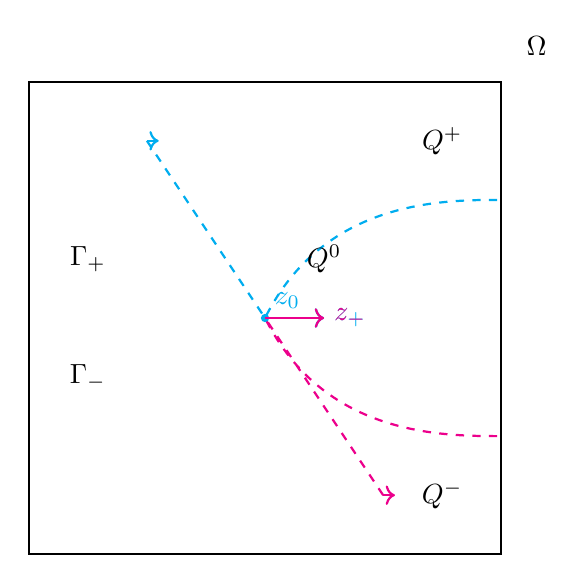
\begin{tikzpicture}[scale=1.5]
        % Define coordinates
        \coordinate (A) at (-2,-2);
        \coordinate (B) at (2,-2);
        \coordinate (C) at (2,2);
        \coordinate (D) at (-2,2);
        
        % Draw the rectangle
        \draw[thick] (A) rectangle (C);
        
        % Define points inside the rectangle
        \coordinate (z+) at (-1, 1.5);
        \coordinate (z0) at (0, 0);
        \coordinate (z-) at (1, -1.5);
        
        % Draw the curves
        \draw[dashed, cyan, thick] (z+) -- (z0) .. controls (0.5, 1) and (1.5, 1) .. (2, 1);
        \draw[dashed, magenta, thick] (z-) -- (z0) .. controls (0.5, -1) and (1.5, -1) .. (2, -1);
        
        % Draw the labels
        \node at (1.5, 1.5) {$Q^+$};
        \node at (1.5, -1.5) {$Q^-$};
        \node at (0.5, 0.5) {$Q^0$};
        
        % Draw the intermediate point
        \fill[cyan] (z0) circle (1pt) node[above right] {$z_0$};
        
        % Draw the arrows
        \draw[->, cyan, thick] (z+) -- ++(0.1, 0);
        \draw[->, magenta, thick] (z-) -- ++(0.1, 0);
        
        % Draw the labels for the curves
        \node at (-1.5, 0.5) {$\Gamma_+$};
        \node at (-1.5, -0.5) {$\Gamma_-$};
        
        % Draw the axes
        \draw[->, cyan, thick] (z0) -- ++(0.5, 0) node[right] {$z_+$};
        \draw[->, magenta, thick] (z0) -- ++(0.5, 0) node[right] {$z_-$};
        
        % Draw the labels for the regions
        \node at (2.3, 2.3) {$\Omega$};
    \end{tikzpicture}
    \caption{Construction of the trajectories. The curve $\Gamma_+$ connects any point $z_+ \in Q^+$ to some intermediate point $z_0 \in Q^0$, whereas the curve $\Gamma_-$ connects any point $z_- \in Q^-$ to some intermediate point $z_0 \in Q^0$.}
    \label{fig:trajectories}
\end{figure}

\end{document}